We validated our methodology by developing a use-case concerning risk assessment for financial companies.
Our application is inspired on the ORCA System\footnote{The ORCA System is a trademark of GCP Global (www.gcpglobal.com).}.
Risk assessment is implemented by an interactive business process based on the exchange of a series of questionnaires intended to evaluate the risks implied the client's business practice.
For instance, the conditions and protocols used to perform confidential transactions, the physical security for accessing reserved areas such as computing server installations.
The information gathered by the questionnaires is used to determine whether there are risky practices within the business processes of the company, as well as to propose amends to these practices.
The ultimate goal of the risk assessment is to determine a degree of compliance to existing standards.
By analysing the questionnaires, ORCA detects risky practices, proposes solutions and triggers further assessment processes to ensure that the solutions have been implemented.

Our goal is to model a service based application (called \FlyingPig), for providing risk assessment as a service.
In order to provide this functionality, \FlyingPig\ would benefit from ORCA's legacy services: storage, assessment and data visualization functions.

In the following, we describe the results of applying $\Pi$-SODM to develop the \FlyingPig\ risk assessment system.
The models presented next were generated as a result of interacting with software developers at GCP Global.

\begin{figure}
\centering
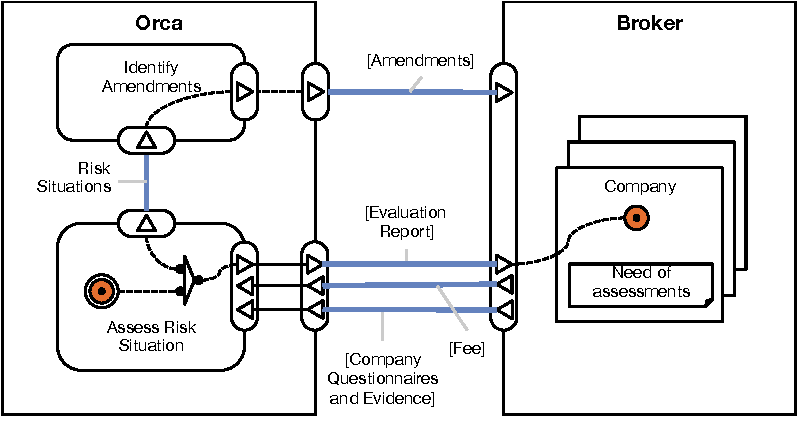
\includegraphics[width=0.7\textwidth]{figs/3ValueModel.pdf}
\hspace*{5cm}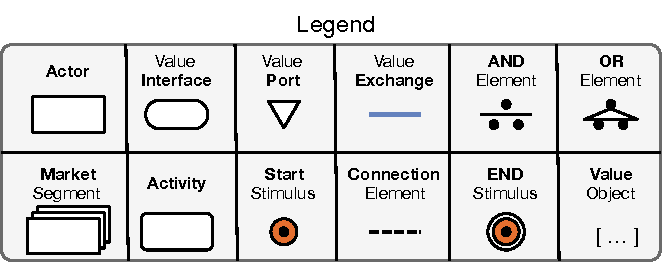
\includegraphics[width=0.4\textwidth]{figs/3ValueKey.pdf}
\caption{E3value model for \FlyingPig.\label{fig:E3valuemodel}}
\end{figure}


\subsection{Computation-Independent Models (CIM)}

$\Pi$-SODM uses two models at the CIM level (see Section~\ref{sec:modelingWithPISODM}): The E3value~\cite{e3value} model and BPMN~\cite{BPMN}.
The former is a simple model just to identify the transference of value information between components of the system.
The BPMN model establishes which are the actors and main tasks of the application.

Figure~\ref{fig:E3valuemodel} shows the value model for the \FlyingPig\ application.
It is a business model that graphically represents a business case as a set of value exchanges ($\triangleright$ and $\triangleleft$) and value activities (rounded boxes) performed by business actors (squared boxes).

In our use-case, we identify two business actors: \textsl{ORCA} and \textsl{Broker}. 
Brokers are responsible for channelling requests for risk assessment of one or several companies. 
ORCA have two value activities which are services that provide an economical benefit: to \textsl{Identify Amendments} and the possibility to \textsl{Assess Risk Situation}. 
The values exchanged between ORCA and the brokers are: \textsl{Amendments} and \textsl{Evaluation Reports} which are value objects ([ \!\dots]) for the companies that need to have a risk assessment, as well as  \textsl{Questionnaire and Evidences} and the risk assessment \textsl{Fee} which are value objects for ORCA System.

The e3value defines \textit{dependency paths}, showing the value exchanges, which are triggered by the occurrence of an end-consumer need (in our case, the need of a risk assessment). 
A dependency path has a direction and consists of a sequence of linked dependency nodes.
A dependency path starts with a \textit{start stimulus} node and ends with an \textit{end stimulus} node (see Legend on Figure~\ref{fig:E3valuemodel}). 
Dependency paths may also contain \textsl{OR} and \textsl{AND} elements (both for initiate and join alternative and parallel paths).

The dependency path in Figure~\ref{fig:E3valuemodel} initiates with the need of assessment by a particular company. 
Once this need occurs, the value exchanges between ORCA and Broker are triggered. 
The client company will provide orca wit information (answers to a questionary), evidence (to support the information) and a fee (monetary value).
ORCA will provide amendments (recommendations to change practices) and an evaluation report. 

\begin{figure}[t]
\centering
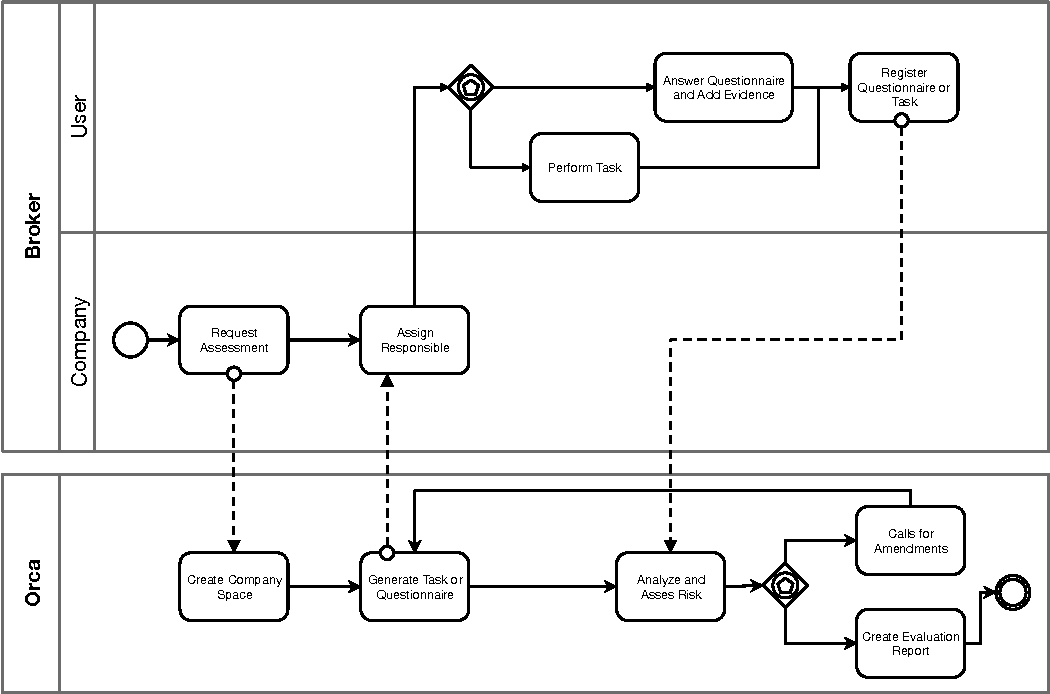
\includegraphics[width=1.0\textwidth]{figs/BPMN_GCP.pdf}

{\color{red} Javier: Please change \underline{Asses} by \underline{Assess}. --M}
\caption{BPMN model for \FlyingPig.\label{fig:BPMNmodel}}
\end{figure}

The BPMN model is devised to better understand the process in which the value exchanges occur.
Figure~\ref{fig:BPMNmodel} shows the BPMN model\footnote{Details on BPMN (Business Process Management Notation) can be found in http://www.bpmn.org/.} for the \FlyingPig\ scenario. 
The model includes two pools representing the \textsl{ORCA} system and the \textsl{Brokers}. 
Brokers have two lanes, the client \textsl{Company} and a \textsl{User}. 
The user is a contact member of the company, who will coordinate the assessment process. 
This process will involve other members of the company as well.

The risk assessment process starts after a request from a company.
(This agrees with the value model, in which the start stimulus triggers the whole process.)
The request leads to the definition of a group of users that will answer questionnaires for evaluating risk.
Questionnaires are considered tasks that users will have to perform. 
Other tasks include amending a ``risky situation'' as well as producing evidence to show that a specific risk has been eliminated\footnote{Risky situations include from physical facts such as not having easy access to handicapped persons or having an unsecured access to the premises of the company, to more intangible ones, such as the use of an less-than-optimal protocol to access data on the company's computer server.}.

Once tasks are completed, they are stored and analysed to generate a list of un-compliant situations, associated to their corresponding \textit{calls for amendment}, in case there are any, or a report specifying a compliance level, incidents and a risk map.
During the process of analysing a questionnaire, the answers of some questions can trigger the generation of other questionnaires or amendments, that will become new tasks.  

Business processes have also associated rules and constraints that define their non functional requirements.
NFR represents the ``semantics'' and the conditions in which the tasks must be done.
In our example we have some constraints.

{\color{red}
Placido, Valeria: What can we say about non-functional requirements at the CIM level?
}



\begin{itemize}
\item {\color{magenta} Placido and Umberto: Could you please complete these items? --G \& M.}
\end{itemize}




\subsection{Platform-Independent Models (PIM)}

In Section~\ref{sec:modelingWithPISODM} we defined three models at the PIM level.
These models are built next, for the \FlyingPig\ scenario.

\begin{figure}[t]
\centering
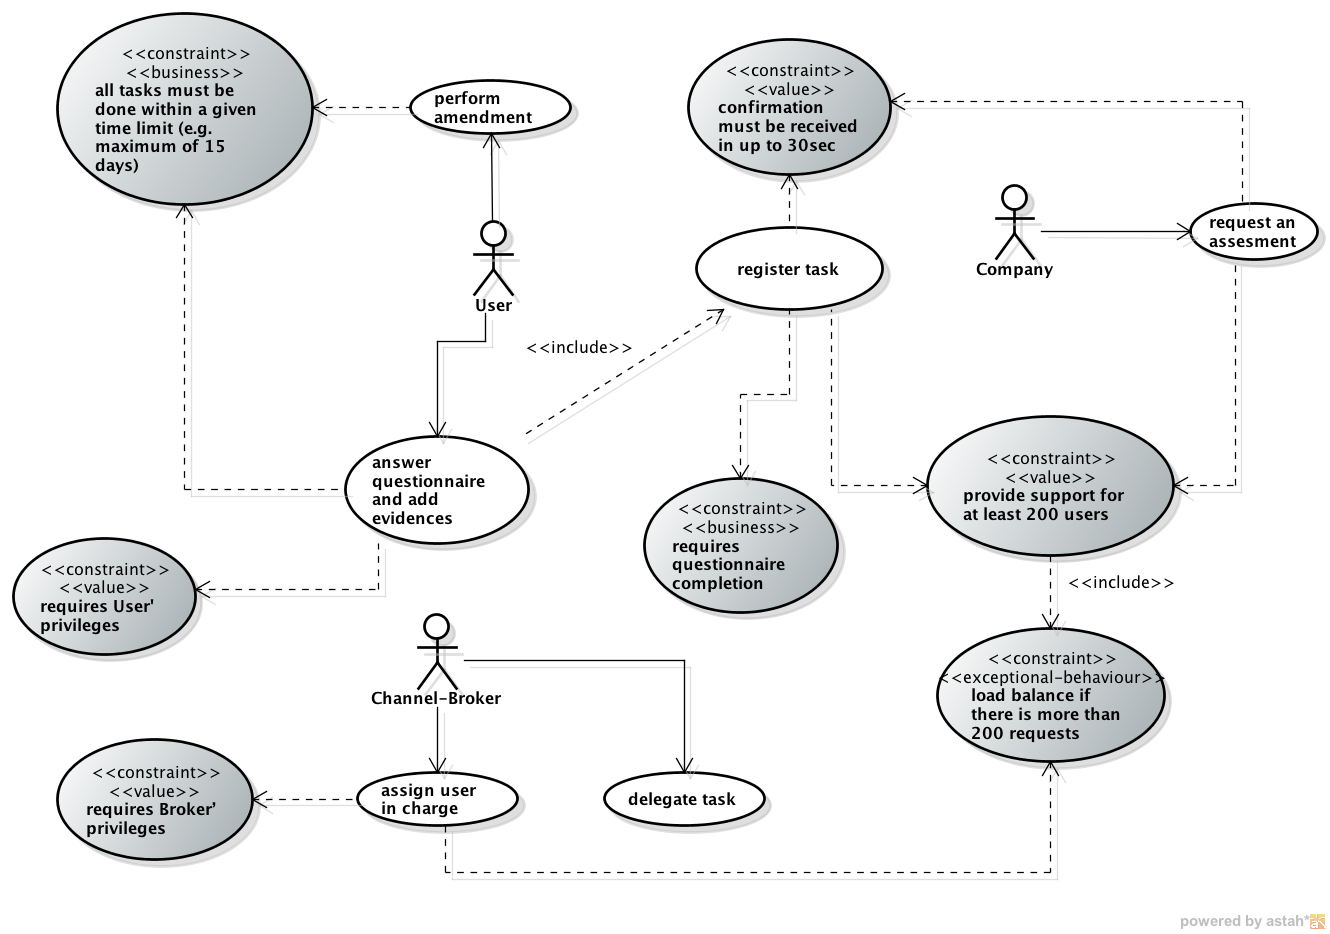
\includegraphics[width=0.9\textwidth]{figs/UseCaseGeneral.png}

{\color{red} 
``Create a responsible'' should be changed for ``Designate user in charge''

``requires concurrency for more than 200 users'' should be changed by ``Maximum number of users should be greater than 200''
}
\caption{$\pi$-UseCase model for \FlyingPig.\label{fig:piUseCaseModel}}
\end{figure}


\paragraph{\underline{$\pi$-UseCase Model for \FlyingPig}}~

The $\pi$-UseCase model shown in Figure~\ref{fig:piUseCaseModel} describes the features and constraints for the \FlyingPig\ application. 
In this model, three actors are identified: \textit{Company}, \textit{User} and \textit{Channel-Broker}\footnote{\color{red} Can we change this for Broker ? --M.}. 
They are represented as stick figures.
In the context of \FlyingPig, Company is the actor asking for risk evaluation.
A Channel-Broker is the responsible for channelling the the evaluation process, assigning users to be in charge of tasks as well as delegating tasks. 
A User, in this model is an actor who answers questionnaires (with base on the actual facts about the Company).
The User also produces evidence to support facts and performs the necessary amendments to improve the results of the risk assessment.

Each actor is associated to one or more use cases (depicted as white ovals in Figure~\ref{fig:piUseCaseModel}). 
Use cases describe the main functionalities of the system.
The $\pi$-UseCase model for \FlyingPig\ defines six use cases. 

In our model, each use case may be associated to one or more (non-functional) constraints (depicted as coloured ovals in Figure~\ref{fig:piUseCaseModel}). 
The model defines three types of constraints: \textit{value} , \textit{business} or \textit{exceptional behavior}. 
Each constraint is identified by the word $<<$\textsf{constraint}$>>$ followed by its type.

In the case of \FlyingPig, the model counts seven constraints:
The use case \textsf{request assessment} has two value constraints.
One of them requires a response time of less than 30 seconds while the other requires that the system's infrastructure should be prepared to deal with, at least 200 users. 

PARE AQUI --Martin

Moreover, an associated constraint requires that if the number of requests exceeds 200 , FlyingPig should make a load balance of the requests. The use case create a responsible has a value constraint ( ii.d ) which defines that the Channel-Broker must have privileges verified before the execution to perform this action. This use case also ( ii.c ) is also related with the load balancing verification. The use case ( iii ) delegate task has no associated constraint . The use case answer questionnaire and add evidences have 2 constraints , they are: the User which performs this action ( iv.e ) must have privileges to answer the questionnaires and ( iv.f ) the time limit must be less than 15 days. The use case register task has 3 constraints associated . Two of them are the same constraints related with the request assessment use case, where (v.a) need a response time confirmation that should be up to 30 seconds, and the other ( v.b ) describes what the system should support a large number of requests for this action, once Users from various companies will be answering the questionnaire and performing tasks. The other constraint requires that ( v.g ) throughout the survey all the questions must be properly answered . Finally , the use case ( vi.f ) perform amendment must be executed in a set time limit in days, the same constraint related with the use case questionnaire answer and add evidences. Figure A presents the relation between the use case and its constraints.








\begin{figure}
\centering
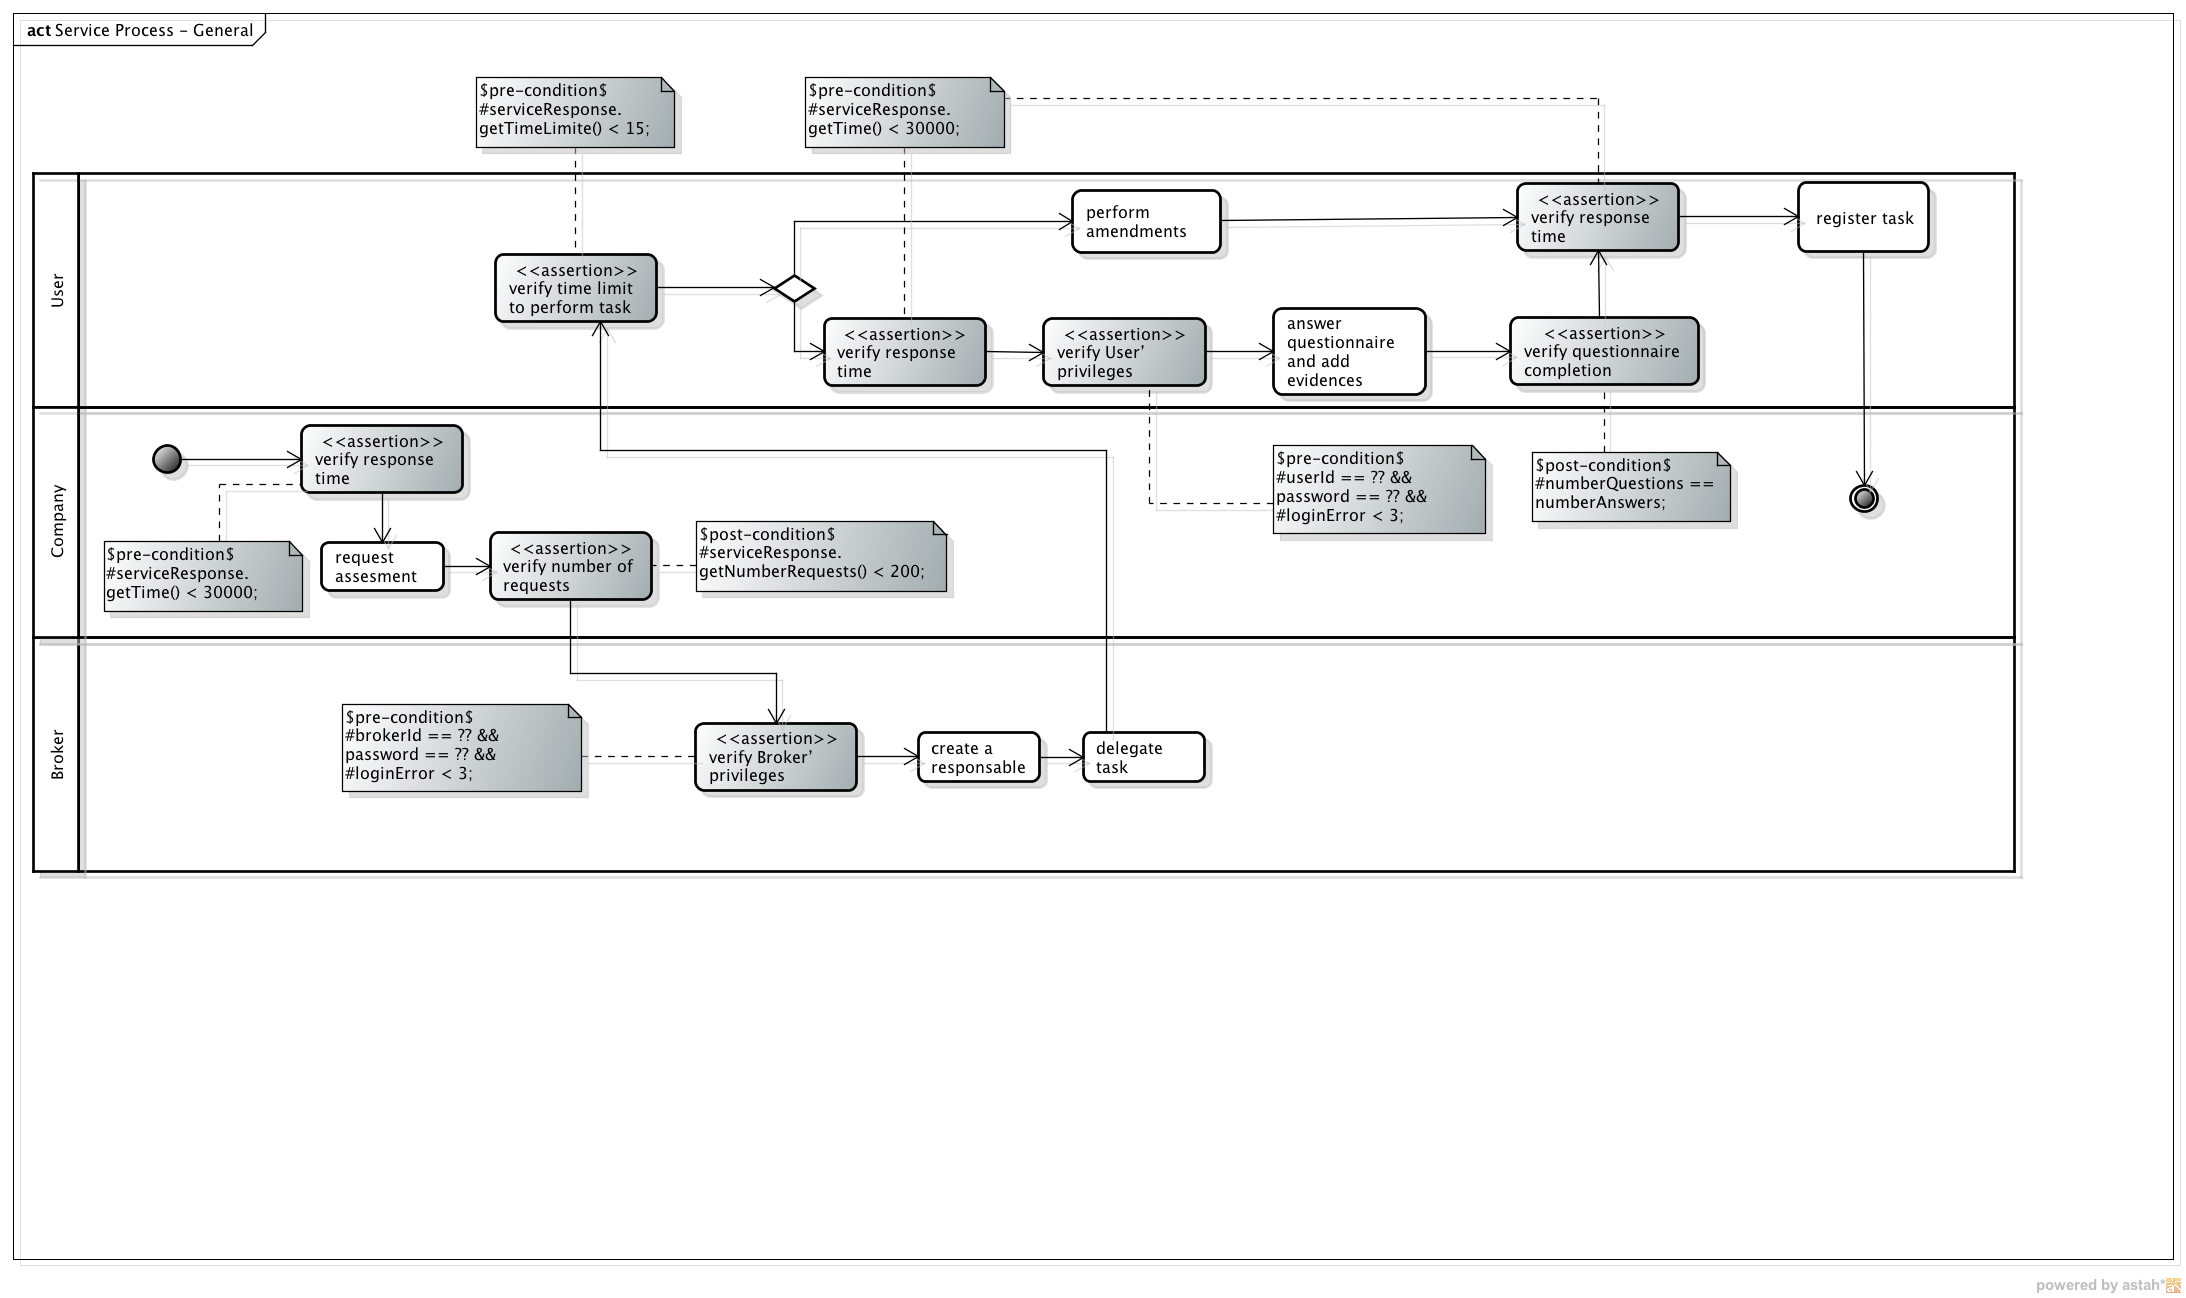
\includegraphics[width=1.0\textwidth]{figs/ServiceProcessGeneral.png}
\caption{$\pi$-ServiceProcess model for \FlyingPig.\label{fig:PiServiceProcessModel}}
\end{figure}

\begin{figure}
\centering
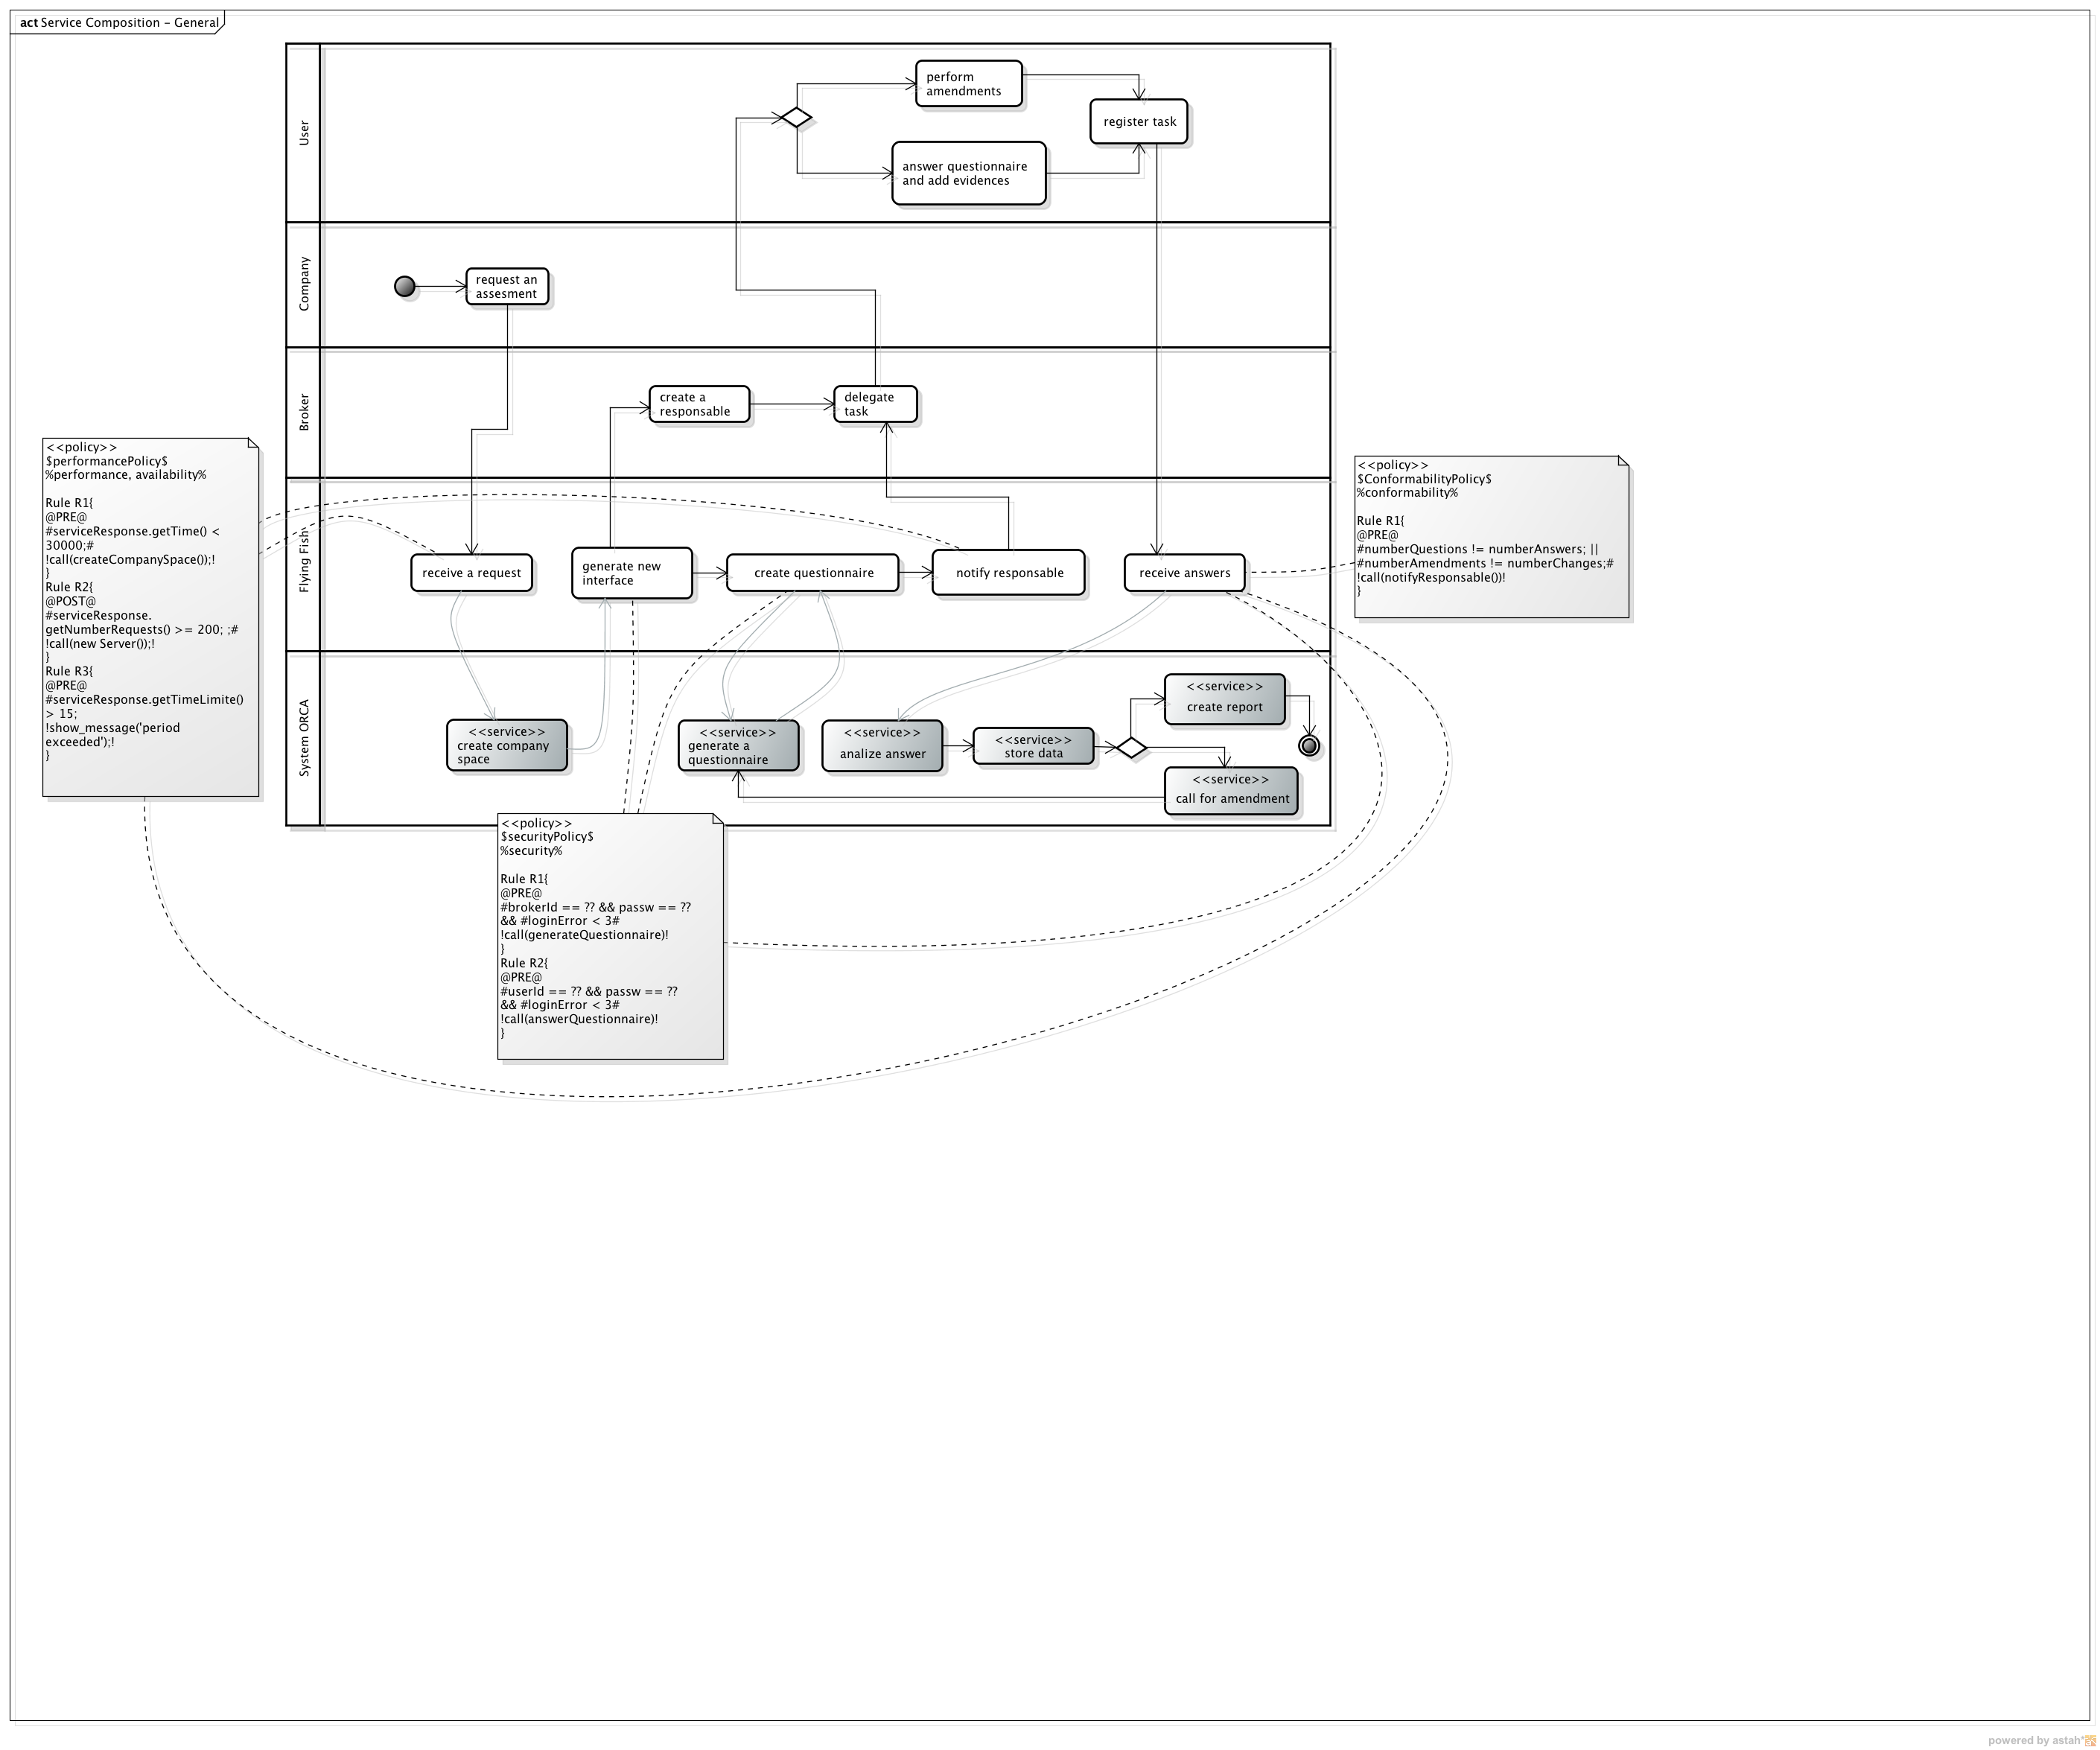
\includegraphics[width=1.0\textwidth]{figs/ServiceCompositionGeneral.png}
\caption{$\pi$-ServiceComposition model for \FlyingPig.\label{fig:PiServiceCompositionModel}}
\end{figure}


\subsection{PSM}

{\color{magenta} Placido and Umberto: Could you please insert the $\pi$-PEWS model here? --G \& M.}


%%%%%%%%%%%%%%%%%%%%%%%%%%%%%%%%%%%%%%%%%%%%%%%%%%5
%% By Placido...
%%%%%%%%%%%%%%%%%%%%%%%%%%%%%%%%%%%%%%%%%%%%%%%%%%

Pi-UseCase Model description for FlyingPig

The piUseCase model shown in Figure  X models the use cases (features) and constrainsts for the FlyingPig application. 3 actors are identified in this model, the are: (I) Company, (II) User and the (III) Channel-Broker. The Company is the whom ask for risk evaluation, the (II) Channel-Broker is the responsible for managing a defining the evaluation flow, beyond create responsible for evaluating and delegate the tasks. This model also represents the (III) User actor which answers questionnaires for the assessment, including evidence and proceeding with necessary corrections when asked for this type of task.

Each actor is associated with use cases. Use cases represent the actions that the actors are responsible. Altogether, this model defines 6 (six) use cases. The use cases related to the Company's actor is (i) request assessment. The use cases related to Broker-Channel's actor are: (ii) create a responsable and (iii) delegate task; and the use cases related User's actor are: (iv) answer questionnaire and add evidences, (v) register task, and (vi) perform amendment.

In this model, each use case may be related with one or more constraints. The constraints can be of three types: value , business or exceptional behavior . This model as a whole has 7 constraints . The use case (i) request assessment has 2 constraints related with, the are from the value type. One is related to ( i.a) response time (confirmation) that should be up to 30 seconds , and the other ( i.b ) describes that the system should support a large number of requests from different companies . Moreover ( i.c ) if the number of requests exceeds 200 , FlyingPig should make a load balance of the requests. The use case create a responsable has a value constraint ( ii.d ) which defines that the Channel-Broker must have privileges verified before the execution to perform this action. This use case also ( ii.c ) is also related with the load balancing verification. The use case ( iii ) delegate task has no associated constraint . The use case answer questionnaire and add evidences have 2 constraints , they are: the User which performs this action ( iv.e ) must have privileges to answer the questionnaires and ( iv.f ) the time limit must be less than 15 days. The use case register task has 3 constraints associated . Two of them are the same constraints related with the request assessment use case, where (v.a) need a response time confirmation that should be up to 30 seconds, and the other ( v.b ) describes what the system should support a large number of requests for this action, once Users from various companies will be answering the questionnaire and performing tasks. The other constraint requires that ( v.g ) throughout the survey all the questions must be properly answered . Finally , the use case ( vi.f ) perform amendment must be executed in a set time limit in days, the same constraint related with the use case questionnaire answer and add evidences. Figure A presents the relation between the use case and its constraints.






TABLE A - RELATION BETWEEN USE CASE AND CONSTRAINT
use cases / constraints	(i) request assessment	(ii) create e responsable 	(iii) delegate task	(iv) answer questionnaire and add evidences	(v) register task	(vi) perform amendment
(a) confirmation must be received in up to 30sec	X				X	
(b) requires concurrency for more than 200 users	X				X	
(c) load balance if there is more than 200 requests	X	X				
(d) requires Broker’ privileges		X				
(e) requires User' privileges				X		
(f) all tasks must be done within a given time limit (e.g. maximum of 15 days)				X		X
(g) requires questionnaire completion					X	


Pi-ServiceProcess Model description for FlyingPig 

The pi-ServiceProcess model (Figure Y) represents the application execution flow of FlyingPig. In this model the action are the result of the use case transformation identified in pi-UseCase model according to their respective actors. The Company, Broker-Channel and User actors are transformed into rays that represent the business collaborators.

The restrictions associated with each use case are transformed into assertions. The set of assertions related to a particular action form the contract for this action. The process of FlyingPig executing begins with the action ( i ) request assessment performed by the Company. This action has one pre-condition regarding the response time and a post-condition concerning the load balance control for the server when it reaches 200 requests. Once the request is made by the Company for risk analysis, the Broker ( ii ) creates responsible for its analysis and ( iii ) delegate the necessary risk assessment. These actions are executed in sequence and has a pre-condition concerning the Broker's privilege. This can only create responsible and delegate the tasks if their authentication datas are correct and if and there was less than 3 requests. The tasks to be performed by the User can be ( iv ) answer questionnaire and add evidences; or ( v) perform amendments. Both the assertion has one pre-condition concerning the time limit for form submission. In this example, we use the limit of 15 days for form submission. If the User is performing the task of answer questionnaire and add evidences, this will have to enter with their authentication data. As postcondition, it is checked if all the answers were answered . The action of perform amendments has no additional verification. Finally, the user registers the tasks performed. This action has response time verification.

This model refines the concepts defined in the pi-UseCase model in order to better describe the assertions and groups them into contracts.


Pi-ServiceComposition Model description for FlyingPig 

This model (presented in Figure Z) describes the interactions of the actions described in pi-ServiceProcess model with the external services. Services are provided through the ORCA system and the access is accomplished by FlyingPig interface. FlyingPig is the point of interaction between the actions described in the precess with the services offered by ORCA. FlyingPig provides an interface with five actions, they are: receive a request, generate new interface, create questionnaire, notify responsable e receive answers.. This interface makes the direct calls for the ORCA' services. The services offered by ORCA are: create space company, generate the questionnaire, analyze answer, data store, call for amendment and create report. These services are called according to the process execution.

With respect to non-functional requirements, the assertions grouped into contract in the pi-ServiceProcess model are transformed into policies in the pi-ServiceComposition model. The policies identified in this case study are: security, performance and conformability policies. Each policy is associated with specific the services and it is verified at the service execution time regarding the specific rule which the sercive is associated with..





%%%%%%%%%%%%%%%%%%%%%%%%%%%%%%%%%%%%%%%%%%%%%%%%%%%%%
\subsection{Lessons Learned}

Through the example we underlined that every application implements functional aspects that describe its application logic.
Recall that an application logic refers to routines that perform the activities to reach the application objective.
Also there are non functional properties derived from NFR. They refer to strategies to be considered for the application execution like: security, isolation, adaptability, atomicity, and more.
These non functional properties must be ensured at execution time, and they are not completely defined within the application logic.

The challenge is to define them and to associate them with the application logic considering that different to existing solutions that suppose that it is possible to access the execution stat of all the components  of an application and that the application has complete control on them, in the case for service oriented applications  the components are autonomous services
API does not necessarily export information about methods dependency (e.g., in the REST protocol);
they do not share their state (stateless).

Given a set of services with their exported methods known in advance or provided by a  service directory, building services' based applications can be  a simple task that implies expressing an application logic as a services' composition. The challenge being  ensuring the compliance between the specification and the resulting application. Software engineering methods (e.g., \cite{1,2,decastro1,PapazoglouH06}) today can help to ensure this compliance, particularly when information systems include several sometimes complex business processes calling Web services or legacy applications exported as services.
